% Generazione delle variabili che andranno a sostituire quelle del template `HomePage.tex`
\newcommand{\documento}{\MU}
\newcommand{\nomedocumentofisico}{\MUv.pdf}
\newcommand{\redazione}{\TG \\ & \CV}
\newcommand{\verifica}{\LC \\ & \NC}
\newcommand{\approvazione}{\SG}
\newcommand{\versione}{1.0.0}
\newcommand{\uso}{Esterno}
\newcommand{\destinateTo}{\TV, \\ & \RC, \\ & \II}
\newcommand{\datacreazione}{02 aprile 2019}
\newcommand{\datamodifica}{02 aprile 2019}
\newcommand{\stato}{Approvato}

\def\TABELLE{true}	% abilita - disabilita l'indice delle tabelle
\def\FIGURE{true} 	% abilita - disabilita l'indice delle figure


\documentclass[a4paper,11pt]{article}

\usepackage{ifthen}
\usepackage[english,italian]{babel}
\usepackage[utf8]{inputenc}
\usepackage[T1]{fontenc}
\usepackage{float}
\usepackage{chapterbib}
\usepackage{graphicx}
\usepackage[a4paper,top=2.5cm,bottom=2.5cm,left=2.5cm,right=2.5cm]{geometry}

\PassOptionsToPackage{hyphens}{url}\usepackage[hyperfootnotes=false]{hyperref}
\hypersetup{%
	colorlinks=true,
	citecolor=black,
	linkcolor=black,
	urlcolor=blue
}

\usepackage{enumitem}
\usepackage{eurosym}
\usepackage{booktabs}
\usepackage{fancyhdr}
\usepackage{totpages}
\usepackage{tabularx, array}
\usepackage{dcolumn}
\usepackage{epstopdf}
\usepackage{booktabs}
\usepackage{fancyhdr}
\usepackage{longtable}
\usepackage{calc}
\usepackage{datatool}
\usepackage[bottom]{footmisc}
\usepackage{listings}
\usepackage{textcomp}
\usepackage{titlesec}
\usepackage{rotating}
\usepackage{multirow}
\usepackage{placeins}
\usepackage{color}
\usepackage{makecell}
\usepackage{lscape}
 
\usepackage[table,usenames,dvipsnames]{xcolor}
% Definizione di nuovi colori da poter usare per le tabelle
\definecolor{lightgray}{gray}{0.92}
\definecolor{lightblue}{rgb}{0.93,0.95,1.0}
\definecolor{headgray}{gray}{0.88}

% Ridefinizione dell'env tabularx. Il vecchio è utilizzabile con l'env oldtabularx
\let\oldtabularx\tabularx
\let\endoldtabularx\endtabularx
\renewenvironment{tabularx}{\rowcolors{2}{white}{lightgray}\oldtabularx}{\endoldtabularx}

% Per tabularx con padding, parametro tra [], eg [1.3]
\newenvironment{paddedtablex}[1][1]{%
	\renewcommand*{\arraystretch}{#1}%
	\renewcommand\theadfont{\bfseries}%
	\tabularx%
}{%
	\endtabularx
}

% Ridefinizione dell'env tabular. Il vecchio è utilizzabile con l'env oldtabular
\let\oldtabular\tabular
\let\endoldtabular\endtabular
\renewenvironment{tabular}{\rowcolors{2}{lightgray}{white}\oldtabular}{\endoldtabular}

% Per tabular con padding, parametro tra [], eg [1.3]
\newenvironment{paddedtable}[1][1]{%
	\renewcommand*{\arraystretch}{#1}%
	\renewcommand\theadfont{\bfseries}%
	\tabular%
}{%
	\endtabular
}

% ***TABELLA ANALISI RISCHI PDP***

\newenvironment{risktable}[1][1]{%
	\centering%
	\renewcommand*{\arraystretch}{1.4}%
	\renewcommand\theadfont{\bfseries}%
	\oldtabularx%
}{%
	\endoldtabularx
}

% ***TABELLA SUDDIVISIONE DEL LAVORO PDP***

\newenvironment{detailtable}[1][1]{%
	\centering%
	\renewcommand*{\arraystretch}{1.4}%
	\renewcommand\theadfont{\bfseries}%
	\oldtabularx%
}{%
	\endoldtabularx
}

% ***TABELLA ORGANIGRAMMA***

\newenvironment{orgtable}[1][1]{%
	\centering%
	\renewcommand*{\arraystretch}{1.4}%
	\renewcommand\theadfont{\bfseries}%
	\oldtabularx%
}{%
	\endoldtabularx
}


% DA SPOSTARE SU COMANDI
% ***DOUBLE LINE***

\def\mydoublerule#1#2#3{%%
	\hrule width#1 height#2 \vskip#2
	\hrule width#1 height#3 
}

% ***NUOVO TIPO DI CELLA CENTRATA***

\newcolumntype{Y}{>{\centering\arraybackslash}X}

% ***STILE PAGINA***
\pagestyle{fancy}

% ***INTESTAZIONE***
\rhead{\Large{\progetto} \\ \footnotesize{\documento}}
\lhead{
\includegraphics[keepaspectratio = true, width = 25px]{../template/icons/a6(1).png}}

% ***PIÈ DI PAGINA***
\lfoot{\textit{\gruppo} \\
\footnotesize{\email}}

\rfoot{\thepage} % per le prime pagine: mostra solo il numero romano
\cfoot{}
\renewcommand{\footrulewidth}{0.4pt}   % Linea sopra il piè di pagina
\renewcommand{\headrulewidth}{0.4pt}  % Linea sotto l'intestazione

% ***INSERIMENTO DI NUOVE SOTTOSEZIONI
\setcounter{secnumdepth}{7} %mostra nel documento fino al livello 8 (1.2.3.4.5.6.7.8)
\setcounter{tocdepth}{7}    % mostra nell'indice fino al livello 8 (1.2.3.4.5.6.7.8)


\makeatletter
\newcounter{subsubparagraph}[subparagraph]
\renewcommand\thesubsubparagraph{%
	\thesubparagraph.\@arabic\c@subsubparagraph}
\newcommand\subsubparagraph{%
	\@startsection{subsubparagraph}    % counter
	{6}                              % level
	{\parindent}                     % indent
	{3.25ex \@plus 1ex \@minus .2ex} % beforeskip
	{0.75em}                           % afterskip
	{\normalfont\normalsize\bfseries}}
\newcommand\l@subsubparagraph{\@dottedtocline{6}{10em}{5.5em}} %gestione dell'indice
\newcommand{\subsubparagraphmark}[1]{}
\makeatother

\makeatletter
\newcounter{subsubsubparagraph}[subsubparagraph]
\renewcommand\thesubsubsubparagraph{%
	\thesubsubparagraph.\@arabic\c@subsubsubparagraph}
\newcommand\subsubsubparagraph{%
	\@startsection{subsubsubparagraph}    % counter
	{7}                              % level
	{\parindent}                     % indent
	{3.25ex \@plus 1ex \@minus .2ex} % beforeskip
	{0.75em}                           % afterskip
	{\normalfont\normalsize\bfseries}}
\newcommand\l@subsubsubparagraph{\@dottedtocline{7}{10em}{6.5em}} %gestione dell'indice
\newcommand{\subsubsubparagraphmark}[1]{}
\makeatother

 % Layout del documento
% Generali
\newcommand{\progetto}{Butterfly}
\newcommand{\gruppo}{AlphaSix}
\newcommand{\email}{alpha.six.unipd@gmail.com}

% Documenti
\newcommand{\AdR}{Analisi dei Requisiti}
\newcommand{\NdP}{Norme di Progetto}
\newcommand{\PdP}{Piano di Progetto}
\newcommand{\SdF}{Studio di Fattibilità}
\newcommand{\PdQ}{Piano di Qualifica}
\newcommand{\VI}{Verbale Interno}
\newcommand{\VE}{Verbale Esterno}
\newcommand{\ST}{Specifica Tecnica}
\newcommand{\DDP}{Definizione di Prodotto}
\newcommand{\MU}{Manuale Utente}
\newcommand{\Gl}{Glossario}
\newcommand{\LdP}{Lettera di Presentazione}
\newcommand{\AdRv}{AnalisiDeiRequisiti v2.0.0}
\newcommand{\NdPv}{NormeDiProgetto v2.0.0}
\newcommand{\PdPv}{PianoDiProgetto v2.0.0}
\newcommand{\PdQv}{PianoDiQualifica v2.0.0}
\newcommand{\SdFv}{StudioDiFattibilità v1.0.0}
\newcommand{\DdPv}{DefinizioneDiprodotto v1.0.0}
\newcommand{\Glv}{Glossario v2.0.0}

% Componenti del gruppo
\newcommand{\LC}{Laura Cameran}
\newcommand{\TG}{Timoty Granziero}
\newcommand{\CV}{Ciprian Voinea}
\newcommand{\SG}{Samuele Gardin}
\newcommand{\NC}{Nicola Carlesso}
\newcommand{\MM}{Matteo Marchiori}

% Ruoli
\newcommand{\RdP}{Responsabile di Progetto}
\newcommand{\Res}{Responsabile}
\newcommand{\Red}{Redattore}
\newcommand{\Amm}{Amministratore}
\newcommand{\Ver}{Verificatore}
\newcommand{\Prog}{Progettista}
\newcommand{\Progr}{Programmatore}
\newcommand{\Ana}{Analista}
\newcommand{\RdPs}{Responsabili di Progetto}
\newcommand{\Ress}{Responsabile}
\newcommand{\Amms}{Amministratori}
\newcommand{\Vers}{Verificatori}
\newcommand{\Progs}{Progettisti}
\newcommand{\Progrs}{Programmatori}
\newcommand{\Anas}{Analisti}

% Professori e proponente
\newcommand{\TV}{Prof. Tullio Vardanega}
\newcommand{\RC}{Prof. Riccardo Cardin}
\newcommand{\LuC}{Luca Cappelletti}
\newcommand{\DZ}{Davide Zanetti}
\newcommand{\II}{Imola Informatica}
\newcommand{\proponente}{Imola Informatica}

% Comando per una nuova riga nella tabella del diario delle modifiche
\newcommand{\specialcell}[2][c]{%
	\begin{tabular}[#1]{@{}c@{}}#2\end{tabular}}

\renewcommand*\sectionmark[1]{\markboth{#1}{}}
\renewcommand*\subsectionmark[1]{\markright{#1}}

% Pediodi di lavoro 
\newcommand{\AR}{Analisi dei Requisiti}
\newcommand{\AD}{Analisi dei Requisiti in Dettaglio}
\newcommand{\PA}{Progettazione Architetturale}
\newcommand{\PD}{Progettazione di Dettaglio}
\newcommand{\CO}{Codifica}
\newcommand{\VV}{Validazione}

% Revisioni
\newcommand{\RR}{Revisione dei Requisiti}
\newcommand{\RP}{Revisione di Progettazione}
\newcommand{\RQ}{Revisione di Qualifica}
\newcommand{\RA}{Revisione di Accettazione}

\newcommand{\myincludegraphics}[2][]{%
	\setbox0=\hbox{\phantom{X}}%
	\vtop{
		\hbox{\phantom{X}}
		\vskip-\ht0
		\hbox{\includegraphics[#1]{#2}}}}

% Ridefinizione linea per le note a piè di pagina
\renewcommand{\footnoterule}{%
  \kern -3pt
  \hrule width \textwidth height 0.4pt
  \kern 2pt
}

\colorlet{punct}{red!60!black}
\definecolor{background}{HTML}{EEEEEE}
\definecolor{delim}{RGB}{20,105,176}
\colorlet{numb}{magenta!60!black}
\lstdefinelanguage{json}{
 	basicstyle=\small\ttfamily,
 	numbers=left,
 	numberstyle=\scriptsize,
 	stepnumber=1,
 	numbersep=8pt,
 	showstringspaces=false,
 	breaklines=true,
 	frame=lines,
 	backgroundcolor=\color{background},
 	literate=
 	*{0}{{{\color{numb}0}}}{1}
 	{1}{{{\color{numb}1}}}{1}
 	{2}{{{\color{numb}2}}}{1}
 	{3}{{{\color{numb}3}}}{1}
 	{4}{{{\color{numb}4}}}{1}
 	{5}{{{\color{numb}5}}}{1}
 	{6}{{{\color{numb}6}}}{1}
 	{7}{{{\color{numb}7}}}{1}
 	{8}{{{\color{numb}8}}}{1}
 	{9}{{{\color{numb}9}}}{1}
 	{:}{{{\color{punct}{:}}}}{1}
 	{,}{{{\color{punct}{,}}}}{1}
 	{\{}{{{\color{delim}{\{}}}}{1}
 	{\}}{{{\color{delim}{\}}}}}{1}
 	{[}{{{\color{delim}{[}}}}{1}
 	{]}{{{\color{delim}{]}}}}{1},
}
\lstset{language=json}
\lstset{literate=%
    {Ö}{{\"O}}1
 	{Ä}{{\"A}}1
 	{Ü}{{\"U}}1
 	{é}{{\"s}}1
 	{è}{{\"e}}1
 	{à}{{\"a}}1
	{ö}{{\"o}}1
}


\definecolor{listinggray}{gray}{0.9}
\definecolor{lbcolor}{rgb}{0.9,0.9,0.9}

\lstset{
  backgroundcolor=\color{lbcolor},
  tabsize=4,
  language=Python,
  captionpos=b,
  frame=single,
  numbers=left,
  numberstyle=\tiny,
  numbersep=5pt,
  breaklines=true,
  showstringspaces=false,
  basicstyle=\footnotesize,
  % identifierstyle=\color{magenta},
  keywordstyle=\bfseries\color[rgb]{0,0,1},
  commentstyle=\color[rgb]{0,0.6,0},
  stringstyle=\color{red}
}

% \definecolor{mygreen}{rgb}{0,0.6,0}
% \definecolor{mygray}{rgb}{0.5,0.5,0.5}
% \definecolor{mymauve}{rgb}{0.58,0,0.82}

% \lstset{ 
%   backgroundcolor=\color{white},   % choose the background color; you must add \usepackage{color} or \usepackage{xcolor}; should come as last argument
%   basicstyle=\footnotesize,        % the size of the fonts that are used for the code
%   breakatwhitespace=false,         % sets if automatic breaks should only happen at whitespace
%   breaklines=true,                 % sets automatic line breaking
%   captionpos=b,                    % sets the caption-position to bottom
%   commentstyle=\color{mygreen},    % comment style
%   deletekeywords={...},            % if you want to delete keywords from the given language
%   escapeinside={\%*}{*)},          % if you want to add LaTeX within your code
%   extendedchars=true,              % lets you use non-ASCII characters; for 8-bits encodings only, does not work with UTF-8
%   firstnumber=1000,                % start line enumeration with line 1000
%   frame=single,	                   % adds a frame around the code
%   keepspaces=true,                 % keeps spaces in text, useful for keeping indentation of code (possibly needs columns=flexible)
%   keywordstyle=\color{blue},       % keyword style
%   language=Octave,                 % the language of the code
%   morekeywords={*,...},            % if you want to add more keywords to the set
%   numbers=left,                    % where to put the line-numbers; possible values are (none, left, right)
%   numbersep=5pt,                   % how far the line-numbers are from the code
%   numberstyle=\tiny\color{mygray}, % the style that is used for the line-numbers
%   rulecolor=\color{black},         % if not set, the frame-color may be changed on line-breaks within not-black text (e.g. comments (green here))
%   showspaces=false,                % show spaces everywhere adding particular underscores; it overrides 'showstringspaces'
%   showstringspaces=false,          % underline spaces within strings only
%   showtabs=false,                  % show tabs within strings adding particular underscores
%   stepnumber=2,                    % the step between two line-numbers. If it's 1, each line will be numbered
%   stringstyle=\color{mymauve},     % string literal style
%   tabsize=2,	                   % sets default tabsize to 2 spaces
%   title=\lstname                   % show the filename of files included with \lstinputlisting; also try caption instead of title
% }

\newcommand{\impl}{\textcolor{Green}{Implementato}}
\newcommand{\implno}{\textcolor{Red}{Non Implementato}}

% G di glossario a pedice, con e senza spazio
\newcommand{\GAlt}{\ped{\tiny{G}}}
\newcommand{\G}{\ped{\tiny{G }}}

% e.g. \gloss{progetto}
\newcommand{\gloss}[1]{%
    {\small \textsc{#1}}\GAlt%
}

% D di documento a pedice, con e senza spazio
% \newcommand{\DAlt}{\ped{\tiny{D}}}
\newcommand{\D}{\ped{\tiny{D}}}

% e.g. \Doc{Norme di Progetto}
\newcommand{\Doc}[1]{\textit{#1}\D}

% Comandi per applicare \Doc con un comando unico
\newcommand{\PdQd}{\Doc{\PdQv}}
\newcommand{\PdPd}{\Doc{\PdPv}}
\newcommand{\NdPd}{\Doc{\NdPv}}
\newcommand{\AdRd}{\Doc{\AdRv}}
\newcommand{\SdFd}{\Doc{\SdFv}}
\newcommand{\Gld}{\Doc{\Gld}}

% Le sottosezioni paragraph, subparagraph ecc.. vengono visualizzate come section
\titleformat{\paragraph}{\normalfont\normalsize\bfseries}{\theparagraph}{1em}{}
\titlespacing*{\paragraph}{0pt}{3.25ex plus 1ex minus .2ex}{1.5ex plus .2ex}

\titleformat{\subparagraph}{\normalfont\normalsize\bfseries}{\thesubparagraph}{1em}{}
\titlespacing*{\subparagraph}{0pt}{3.25ex plus 1ex minus .2ex}{1.5ex plus .2ex}

\titleformat{\subsubparagraph}{\normalfont\normalsize\bfseries}{\thesubsubparagraph}{1em}{}
\titlespacing*{\subsubparagraph}{0pt}{3.25ex plus 1ex minus .2ex}{1.5ex plus .2ex}

\titleformat{\subsubsubparagraph}{\normalfont\normalsize\bfseries}{\thesubsubsubparagraph}{1em}{}
\titlespacing*{\subsubsubparagraph}{0pt}{3.25ex plus 1ex minus .2ex}{1.5ex plus .2ex}


% Indentazione paragrafi rimossa. Per metterla manualmente, precedere il paragrafo con il comando /indent
\newlength\tindent
\setlength{\tindent}{\parindent}
\setlength{\parindent}{0pt}
\renewcommand{\indent}{\hspace*{\tindent}}


% Generazione automatica dei numeri per le versioni
\newcounter{vX} % valore per X in X.Y.Z
\newcounter{vY} % valore per Y in X.Y.Z
\newcounter{vZ} % valore per Z in X.Y.Z
\newcommand{\decrvX}{\addtocounter{vX}{-1}} % Comando per il decremento automatico del counter vZ
\newcommand{\decrvY}{\addtocounter{vY}{-1}} % Comando per decrementare vY
\newcommand{\decrvZ}{\addtocounter{vZ}{-1}} % Comando per decrementare vZ
\newcommand{\addToDiary}[4]{\thevX.\thevY.\thevZ & #1 & #2 & #3 & #4\decrvZ\\} % Comando per generare una riga di diario delle modifiche (\addToDiary{desc}{ruolo}{nominativo}{data})

% Colore righe grigie
\newcommand{\tablegray}{gray!20}

% Stile liste
% \renewcommand\labelitemi{$\circ$} % Bullet, primo livello
% \renewcommand\labelitemii{$\diamond$} % Bullet, primo livello
% \renewcommand\labelitemii{\normalfont\bfseries \textendash} % --, secondo livello
% \renewcommand\labelitemiii{\textasteriskcentered} % *, terzo livello
% \renewcommand\labelitemiv{\textperiodcentered} % ., quarto livello
% \setlist[itemize,2]{label=$\circ$}
% \setlist[itemize,2]{label=$\diamond$}

% Placeholder sui diari
\newcommand{\pl}{Placeholder}

%Comandi per le versioni delle tecnologie
\newcommand{\python}{Python 3.6.7}
\newcommand{\gitlab}{GitLab 11.7}
\newcommand{\redmine}{Redmine 4.0.1}
\newcommand{\kafka}{Apache Kafka 2.12}
\newcommand{\docker}{Docker 18.09}
\newcommand{\telegram}{Telegram (Bot API 4.0)}
\newcommand{\slack}{Slack}
\newcommand{\jenkins}{Jenkins 2.146}


 % Comandi generali

\newcommand{\lettera}[1]{
  % \newpage
  \rule{\textwidth}{0.4pt}
  \invisiblesection{#1}
  \begin{center}
    {\Huge #1} \\
  \end{center}
  \vspace{0.9cm}
}

\newcommand\invisiblesection[1]{%
  \refstepcounter{section}
  \addcontentsline{toc}{section}{\protect\numberline{}#1}%
  \sectionmark{#1}
}

\newcommand\invisiblesubsection[1]{%
  \refstepcounter{subsection}%
  \addcontentsline{toc}{subsection}{\protect\numberline{}#1}%
  \sectionmark{#1}
}

\newcommand{\parola}[2]{
  \invisiblesubsection{#1}
  \textbf{\large{#1}} \\
  #2
  \vspace{0.3cm}
}

% no indentazione paragrafo
\setlength{\parindent}{0pt}
 % Comandi del documento

\addtocounter{vZ}{1}
\newcommand{\modifiche}
{
	% \addToDiary{Inserimento qualità di processo}{\Ver}{\NC}{03-01-2018}
	% \addToDiary{Inserimento qualità di prodotto}{\Ver}{\NC}{30-12-2018}
	% \addToDiary{Inserimento standard ISO 90003}{\Ver}{\NC}{27-12-2018}
	% \addToDiary{Inserimento standard ISO 9126}{\Ver}{\NC}{26-12-2018}
	% \addToDiary{Inserimento standard ISO 15504}{\Ver}{\NC}{23-12-2018}
	
	\addToDiary{Aggiunto appendice \S{C} (mitigazione variazioni)}{\Ver}{\MM}{14-02-2019}

	% 1.Y.Z
	\setcounter{vX}{1}%
	\setcounter{vY}{0}%
	\setcounter{vZ}{0}%

	\addToDiary{Approvazione per il rilascio}{\Res}{\NC}{13-01-2019}

	% 0.2.Z
	\decrvX
	\setcounter{vY}{2}%
	\setcounter{vZ}{0}%

	\addToDiary{Verifica finale}{\Ver}{\MM}{12-01-2019}

    % 0.1.Z
    \decrvY%
	\setcounter{vZ}{2}%

	\addToDiary{Aggiunto appendice ``Valutazioni per il miglioramento''}{\Ver}{\MM}{11-01-2019}
	\addToDiary{Inserito ``Resoconto delle attività di verifica''}{\Ver}{\NC}{08-01-2019}
	\addToDiary{Verifica documento}{\Ver}{\CV}{10-12-2018}

    % 0.0.Z
	\setcounter{vZ}{5}%
	\decrvY%

	\addToDiary{Aggiunto appendice ``Standard di qualità''}{\Ver}{\NC}{03-12-2018}
	\addToDiary{Inserito ``Qualità di processo''}{\Ver}{\NC}{02-12-2018}
	\addToDiary{Inserito ``Qualità di prodotto''}{\Ver}{\TG}{01-12-2018}
	\addToDiary{Aggiunta Introduzione}{\Ver}{\NC}{29-11-2018}
    \addToDiary{Creazione template}{\Red}{\TG}{27-11-2018}
}
 % Entries diario

\begin{document}
	% \sloppy
    % Inclusione template HomePage
    \begin{center}

%\includegraphics[width=1em]{../../../Template/icone/LogoGruppo.png}
\begin{large} \textbf{\progetto} \end{large}
%\includegraphics[width=1em]{../../../Template/icone/LogoGruppo.png}
\vspace{0.2em}

\hrule
\vspace{7em}


\includegraphics[keepaspectratio = true, width=5cm]{../template/icons/sotto.png}

%Prima pagina senza intestazione né piè di pagina	
\thispagestyle{empty}

%spazio tra il nome e il logo
\vspace{1.5em}

%Copertina
\begin{center} 
  \begin{Huge}
  {\fontsize{15mm}{20mm}\selectfont \gruppoLink} 
  \end{Huge}
\end{center}

%Le informazioni del documento sono ancorate a fine pagina
\vfill

\begin{Huge} \documento \end{Huge}

\begin{center}
% \textbf{Informazioni sul documento} \\ \vspace{2em}
% \small
\begin{tabular}{r|l}
	\multicolumn{2}{c}{\textbf{Informazioni sul documento} } \\ \hline
	\textbf{Nome Documento} & \nomedocumentofisico \\
	% \textbf{Versione} & \versione \\
	\textbf{Data di Creazione} & \datacreazione \\
	\textbf{Data ultima modifica} & \datamodifica \\
	\textbf{Stato} & \stato \\
	\textbf{Redazione} & \redazione \\
	\textbf{Verifica} & \verifica \\
	\textbf{Approvazione} & \approvazione \\
	\textbf{Uso} & \uso \\
	\textbf{Distribuzione} & \gruppo \\
	\textbf{Destinato a} & \destinateTo \\
	\textbf{Email di riferimento} & \email
\end{tabular}
\end{center}

\normalsize

% Sommario
\textbf{Descrizione} \\
Questo documento fornisce la definizioni di alcuni dei termini apparsi in altri documenti allegati redatti 
da \gruppo\ durante lo svolgimento del progetto Butterfly, con
lo scopo di evitare ogni forma di ambiguit\`a.
 

%\vfill
\end{center}

\clearpage

    % Registro delle modifiche e indice
    % si usa la numerazione romana per gli indici e la tabella delle modifiche
    \pagenumbering{Roman}
    \addtocounter{vZ}{1}
\newcommand{\modifiche}
{
	% \addToDiary{Inserimento qualità di processo}{\Ver}{\NC}{03-01-2018}
	% \addToDiary{Inserimento qualità di prodotto}{\Ver}{\NC}{30-12-2018}
	% \addToDiary{Inserimento standard ISO 90003}{\Ver}{\NC}{27-12-2018}
	% \addToDiary{Inserimento standard ISO 9126}{\Ver}{\NC}{26-12-2018}
	% \addToDiary{Inserimento standard ISO 15504}{\Ver}{\NC}{23-12-2018}
	
	\addToDiary{Aggiunto appendice \S{C} (mitigazione variazioni)}{\Ver}{\MM}{14-02-2019}

	% 1.Y.Z
	\setcounter{vX}{1}%
	\setcounter{vY}{0}%
	\setcounter{vZ}{0}%

	\addToDiary{Approvazione per il rilascio}{\Res}{\NC}{13-01-2019}

	% 0.2.Z
	\decrvX
	\setcounter{vY}{2}%
	\setcounter{vZ}{0}%

	\addToDiary{Verifica finale}{\Ver}{\MM}{12-01-2019}

    % 0.1.Z
    \decrvY%
	\setcounter{vZ}{2}%

	\addToDiary{Aggiunto appendice ``Valutazioni per il miglioramento''}{\Ver}{\MM}{11-01-2019}
	\addToDiary{Inserito ``Resoconto delle attività di verifica''}{\Ver}{\NC}{08-01-2019}
	\addToDiary{Verifica documento}{\Ver}{\CV}{10-12-2018}

    % 0.0.Z
	\setcounter{vZ}{5}%
	\decrvY%

	\addToDiary{Aggiunto appendice ``Standard di qualità''}{\Ver}{\NC}{03-12-2018}
	\addToDiary{Inserito ``Qualità di processo''}{\Ver}{\NC}{02-12-2018}
	\addToDiary{Inserito ``Qualità di prodotto''}{\Ver}{\TG}{01-12-2018}
	\addToDiary{Aggiunta Introduzione}{\Ver}{\NC}{29-11-2018}
    \addToDiary{Creazione template}{\Red}{\TG}{27-11-2018}
}

    % Inserisce il link all'indice
% \addcontentsline{toc}{section}{Indice}

\tableofcontents
\clearpage 

% Se è stata impostata a true la variabile per la lista delle tabelle, la mostra
\ifthenelse{\equal{\TABELLE}{true}} 
{\listoftables}{}

% Se è stata impostata a true la variabile per la lista delle figure, la mostra
\ifthenelse{\equal{\FIGURE}{true}}
{\listoffigures}{}

% Da qui comincia la numerazione normale
\pagenumbering{arabic}
\setcounter{page}{1}

% Imposta il formato di visualizzazione
\rfoot{\thepage~di~\pageref{TotPages}}

    % Sezioni documento
    \newpage
\section{Introduzione} \label{Introduzione}
	
	\subsection{Scopo del documento}
	Questo \gloss{documento} ha l'intento di specificare la \gloss{pianificazione} e l'approccio che \gruppo\ adotterà per portare a termine il \gloss{progetto} Butterfly.
	All'interno vengono illustrate le strategie, le suddivisioni dei compiti, l'utilizzo delle risorse, la gestione dei rischi e le attività secondo le quali il team di sviluppo ha intenzione di lavorare.
	
	
    \subsection{Scopo del prodotto}

%%| Ex Norme di Progetto |%%
% Il prodotto che \gruppo\ si incarica di realizzare è Butterfly: un \gloss{tool} di supporto alle figure di	sviluppo di aziende di software
% (non solamente quella committente). Questo applicativo permette di incanalare le notifiche dei vari strumenti utilizzati nel percorso di
% \gloss{CI/CD} (come \gloss{Redmine}, \gloss{GitLab}, ecc.) di un software e, tramite un \gloss{Broker} (\gloss{Apache Kafka} in questo caso),
% spedirli alla persona interessata tramite canale di comunicazione preferito scelto da quest’ultimo (email, \gloss{Telegram}, \gloss{Slack}, ecc).

% \vspace{1cm}

%%| Ex Analisi dei Requisiti |%%
Lo scopo del \gloss{prodotto} è creare un \gloss{applicativo} per poter gestire i messaggi o le segnalazioni provenienti da diversi prodotti per la realizzazione di software,
come \gloss{Redmine}, \gloss{GitLab} e opzionalmente \gloss{SonarQube}, attraverso un \gloss{Broker} che possa incanalare questi messaggi e distribuirli a strumenti come
\gloss{Telegram}, e-mail e opzionalmente \gloss{Slack}.\par
Il software dovrà inoltre essere in grado di riconoscere il \gloss{Topic} dei messaggi in input per poterli inviare in determinati canali a cui i
destinatari dovranno iscriversi.\par
\`E anche richiesto di creare un canale specifico per gestire le particolari esigenze dell'azienda. Dovrà essere in grado, attraverso la lettura di
particolari	\gloss{metadati}, di reindirizzare i messaggi ricevuti al destinatario più appropriato.

% \vspace{1cm}

%%| Ex Piano di Qualifica |%%
% Il prodotto finale consiste in uno strumento in grado di ricevere messaggi o segnalazioni da vari tipi di servizi per la produzione software chiamati
% \gloss{producer} (e.g. \gloss{GitLab}, \gloss{Redmine} e \gloss{SonarQube}), per poterli poi incanalare verso altri servizi chiamati \gloss{Consumer}
% atti a notificare gli sviluppatori (e.g. \gloss{Slack}, \gloss{Telegram} e Email).\par    
% L'applicazione sarà inoltre capace di organizzare le segnalazioni suddividendole per topic a cui i vari utenti dovranno iscriversi per esserne notificati.
% Nel caso in cui il destinatario dovesse segnalare di non essere disponibile, l'applicativo deve reindirizzare il messaggio verso la persona di competenza
% più prossima. 

% \vspace{1cm}

%%| Ex Piano di Progetto |%%
% Il prodotto che \gruppo\ si incarica di realizzare è Butterfly: un tool di supporto alle figure di sviluppo in aziende che producono software (non
% solamente quella del committente).
% Questo applicativo permette di incanalare le notifiche dei vari strumenti utilizzati nel percorso di \gloss{CI} e \gloss{CD} (come Redmine,
% GitLab, ecc.) di un software e, tramite un \gloss{broker} (\gloss{Apache Kafka} in questo caso), spedirli alla persona interessata tramite
% il canale di comunicazione preferito scelto da quest'ultimo (email, Telegram, Slack, ecc.).


	\subsection{Glossario e documenti esterni}
Al fine di rendere il documento più chiaro possibile, i termini che possono assumere un significato ambiguo o i riferimenti a documenti esterni
avranno delle diciture convenzionali:

\begin{itemize}
    \item \textbf{D}: indica che il termine si riferisce al titolo di un particolare documento (ad esempio \Doc{\PdPv});
    \item \textbf{G}: indica che il termine si riferisce ad una voce riportata nel \Doc{\Glv} (ad esempio \gloss{Redmine}).
\end{itemize}

	\subsection{Riferimenti}
		\subsubsection{Riferimenti Normativi}
			\begin{itemize}
				\item \NdPd
				\item Capitolato d'appalto C1:\\
				\url{https://www.math.unipd.it/~tullio/IS-1/2018/Progetto/C1.pdf}
				\item Vincoli di organigramma e specifiche economiche\\
				\url{https://www.math.unipd.it/~tullio/IS-1/2018/Progetto/RO.html}
				\item The Twelve-Factor App, norme per lo sviluppo di un prodotto software consigliate dall'azienda.\\
				\url{https://12factor.net/}
			\end{itemize}
		
		\subsubsection{Riferimenti Informativi}\label{rifinfo}
			\begin{itemize}
				\item Software Engineering - Ian Sommerville - 10 th Edition (2016)
				\item Slide dell’insegnamento Ingegneria del Software\\
				\url{http://www.math.unipd.it/~tullio/IS-1/2018/}
				\item I sistemi per la gestione dei rischi (presentazione rilasciata dalla Bocconi per la gestione dei rischi).\\
				\url{https://www2.deloitte.com/content/dam/Deloitte/it/Documents/risk/Board\%20Academy\%20Corso\%20C6\%2020\%20dic\%202012\%20SDA\%20Bocconi.pdf}
				\item Fonte Figura \ref{fig:modello_incrementale}:\\
				\url{https://it.wikipedia.org/wiki/Modello_incrementale}
			\end{itemize}
		
	\subsection{Scadenze}\label{Scadenze}
	\gruppo\ ha deciso di rispettare le scadenze indicate dal professor Vardanega, riportate di seguito:
	\begin{itemize}
		\item \textbf{Revisione dei Requisiti}: 21-01-2019
		\item \textbf{Revisione di Progetto}: 15-03-2019
		\item \textbf{Revisione di Qualifica}: 19-04-2019
		\item \textbf{Revisione di Accettazione}: 17-05-2019.
	\end{itemize}
	
	\subsection{Modello di sviluppo} % Usare modello di sviluppo come termine al posto di Ciclo di vita in questo contesto. Vedere #26
	Data la natura del progetto, composto da più parti modulari e con un basso valore di accoppiamento, si è scelto di adottare un \gloss{modello di
	sviluppo} ibrido tra quello a componenti e quello incrementale.
	Essi si adattano particolarmente bene a questo tipo di progetto, in quanto:
	\begin{itemize}
		\item Il modello incrementale prevede ripetizioni identificate come cicli di incremento che verranno ripetute fino a quando il prodotto non arriverà a soddisfare i \gloss{requisiti} richiesti dal cliente
		\item Il modello a componenti è basato sul riuso di unità software che possono avere diverse dimensioni:
		\begin{itemize}
			\item \textbf{System reuse}: un intero sistema, composto da più applicazioni, può essere riusato come parte di un sistema di tanti sistemi % TODO: rivedere la frase
			\item \textbf{Application reuse}: un'applicazione può essere riusata incorporandola in altri sistemi senza apportare cambiamenti, 
				oppure configurandola
			\item \textbf{Component reuse}: i \gloss{componenti} di un'applicazione, che possono essere da sotto-sistemi a singoli oggetti, risiedono
				in un cloud o in server privati e possono essere accessibili tramite \gloss{Application Programming Interface} (API)
			\item \textbf{Object and function reuse}: componenti software che implementano una singola funzione o una classe oggetto. Si 
				possono riusare collegandole con lo sviluppo di nuovo codice. Molte di queste sono liberamente disponibili. 
		\end{itemize}
		Oppure, nel caso in cui le componenti siano così specifiche da essere troppo costoso adattarle ad una nuova situazione,
		è possibile fare "concept reuse", ovvero riusare le idee che stanno alla base del componente (e.g. riusare un \gloss{way of working} o un algoritmo). \par
		In particolare, i benefici che si possono trarre dal riuso sono:
		\begin{itemize}
			\item \textbf{Costo complessivo di sviluppo più basso}: perché il numero di componenti software che devono essere progettati, implementati e validati è minore.
			\item \textbf{Sviluppo accelerato}
			\item \textbf{Aumento dell'affidabilità}: un software che è stato provato e testato in altri sistemi risulta più affidabile di un software appena implementato.
			Buona parte dei suoi difetti di progettazione e implementazione dovrebbero già esser stati individuati e corretti.
			%\item  Ridotto rischio di processo, vero specialmente per grandi componenti software riusate come sottosistemi. È un fattore importante per il Project Manager perché riduce il margine di errore nella stima dei costi di un progetto.
			\item \textbf{Conformità con gli standard}: alcuni standard
			%, come gli interface standard, 
			possono essere implementati come set di componenti riusabili.
		\end{itemize}
		%e prevede che venga riutilizzata una base per lo sviluppo dei vari pezzi che formano il progetto, fra loro indipendenti
	\end{itemize}
	Inizialmente si possono spendere le risorse nella realizzazione di una base di partenza per le componenti, che verrà successivamente sviluppata per ciascun requisito richiesto, rappresentando il nucleo del prodotto finale.
	A tale \gloss{milestone} si potranno integrare le funzionalità secondarie richieste dal cliente insieme ai possibili requisiti impliciti desiderabili presenti nel capitolato. In base alla pianificazione svolta, le risorse disponibili saranno ridistribuite in modo da garantire lo sviluppo completo del prodotto.
	L'immagine che segue rappresenta il modello incrementale e come il progetto viene composto da componenti sviluppati ciascuno secondo cicli con fasi ben definite.
	\begin{figure}[H]
		\centering
		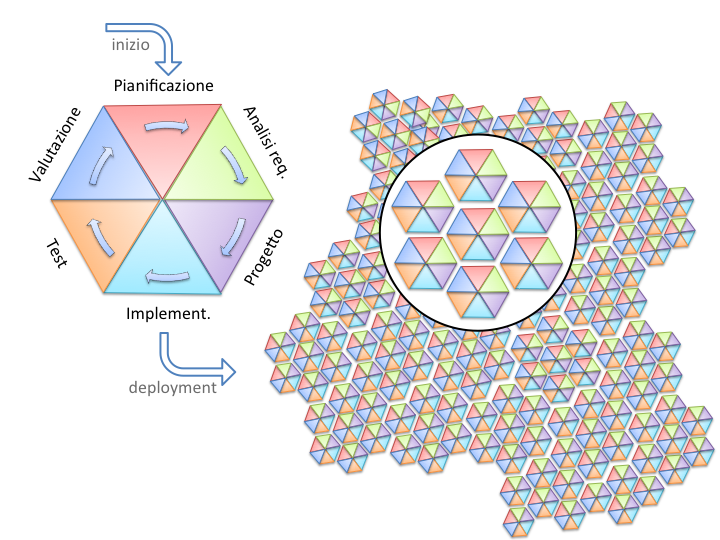
\includegraphics[scale=0.5]{img/modello_incrementale.png}
		\caption{Rappresentazione del modello incrementale\protect\footnotemark}
		\label{fig:modello_incrementale}
	\end{figure}

	\footnotetext{Fonte in \S\ref{rifinfo}}
	
    \section{Configurazione}\label{configurazione}

Su richiesta di \II, tutti i servizi sono stati configurati sotto forma di container. È quindi possibile avviarli su macchine fisiche differenti, ma collegate in rete fra loro, con Docker.\\
Sempre sotto richiesta di \II viene utilizzato Rancher come software per la gestione dei container, quindi questa guida verterà principalmente sulla configurazione di \progetto utilizzando Rancher. %TODO riverere frase per ripetizione

\subsection{Requisiti di sistema}

	Non sono necessari particolari requisiti in modo da poter configurare e utilizzare il nostro prodotte, tuttavia valgono i requisiti minimi dei sistemi di terze parti che vengono utilizzati da \progetto.

	\subsubsection{Software}
		\begin{itemize}
			\item Docker\footnote{\url{https://docs.docker.com/v17.09/datacenter/ucp/2.1/guides/admin/install/system-requirements}}: è necessario avere installata e configurata correttamente almeno la versione v18.09.
			\item Docker Compose\footnote{\url{https://docs.docker.com/compose/install/}} :  nel caso si decidesse di utilizzare Docker Compose per l'avvio dei container è consigliata l'installazione e configurazione corretta della versione v3.7.
			\item Kubernetes\footnote{\url{https://kubernetes.io/docs/setup/independent/install-kubeadm}}: nel caso si decidesse di utilizzare Kubernetes per la gestione dei container è consigliata l'installazione e configurazione corretta della versione v1.13.
			\item Rancher\footnote{\url{https://rancher.com/docs/rancher/v2.x/en/installation/requirements/}}: nel caso si decidesse di utilizzare Rancher per la gestione grafica di oggetti Kubernetes contenenti i container Docker, è consigliata l'installazione e configurazione della versione v2.1.4.
			\item Kafka\footnote{\url{https://docs.confluent.io/current/installation/system-requirements.html}}: è necessario avere installata e configurata correttamente almeno la versione v2.12.
			\item GitLab\footnote{\url{https://git.ucd.ie/help/install/requirements.md}} 11.7
			\item Redmine\footnote{\url{https://www.easyredmine.com/faq/technical-info/176-hardware-and-software-requirements-for-server-solution}}: durante lo sviluppo di \progetto abbiamo utilizzato 4.0.1
		\end{itemize}
	
	%TODO rivedere
	GitLab e Redmine sono componenti esterne a \progetto, tuttavia vengono citate in quanto è possibile configurare tutto il progetto in un ambiente unico.\\
	Le versioni specificate possono essere trovate anche nella sezione ``Requisiti di vincolo'' del documento \AdRv.
	
	\subsubsection{Hardware}
	Per \progetto~non sono necessari ulteriori requisiti a livello hardware particolari se non quelli di cui hanno bisogno i software precedentemente elencati.

\subsection{Mappatura delle porte}
Per la configurazione di ciascun tipo servizio abbiamo deciso di dare un range di porte da poter esporre in modo tale da effettuare una separazione a logico.\\
Questa regola non influisce col corretto funzionamento di \progetto ma è solamente per non assegnare le porte in modalità casuale e facilitare le analisi di eventuali errori come anche la facile manutenzione e aggiunta di servizi.

La suddivisione delle porte è la seguente:

\begin{table}[H]
	\centering
	\begin{paddedtablex}[1.3]{\textwidth}{YYY}
		\thead{Servizio} & \thead{Porta inizio} & \thead{Porta fine}\\\toprule
		Software di terze parti& 30000& 30029\\\hline
		Kafka e servizi correlati& 30030& 30059\\\hline
		Producer& 30060& 30089\\\hline
		Consumer& 30090& 30119\\\hline
		Gestore personale& 30120& 30149\\
	\end{paddedtablex}
	\caption{Suddivisione delle porte}
\end{table}

La suddivisione che abbiamo utilizzato durante lo sviluppo ed alla consegna del progetto prevede la seguente esposizione delle porte:

\begin{table}[H]
	\centering
	\begin{paddedtablex}[1.3]{\textwidth}{YYY}
		\thead{Servizio} & \thead{Porta interna} & \thead{Porta esposta}\\\toprule
		Redmine& 3000& 30000\\\hline
		GitLab& 80& 30001\\\hline
		Kafka& 9092& 30030\\\hline
		Producer GitLab& 5000& 30060\\\hline
		Producer Redmine& 5000& 30061\\\hline
		Consumer Telegram& 30090& \\\hline
		Consumer Email& 30091& \\\hline
		Producer Gestore personale& 30120& 5000\\\hline
		Consumer Gestore personale& 30121& \\
	\end{paddedtablex}
	\caption{Configurazione delle porte in fase di sviluppo e consegna}
\end{table}

Le specifiche relative alla configurazione delle porte in Rancher possono essere trovate nella pagina dedicata\footnote{\url{https://rancher.com/docs/rancher/v2.x/en/installation/references/}} sulla sezione della documentazione presente nel loro sito.

\subsection{Configurazione servizi principali container}

	\subsection{Webhook}
	Per il corretto invio dei webhook (in formato JSON) da parte dei software che comunicano con i nostri Producer è necessaria una piccola configurazione:
	
	\paragraph{Redmine}
	
		\subparagraph{Configurazione del plugin}
	
		scaricarlo nella cartella... 
		verificare in sezione admin in configurazioni parte amministratore...
	
	L'implementazione per Redmine si appoggia sul plugin \texttt{redmine\_webhook}, raggiungibile al link
	\url{https://github.com/suer/redmine_webhook}.
	
	Questo plugin implementa il concetto di Hook offerto dalla API di Redmine, inviando a un determinato URL
	un \gloss{payload} costituito da un file JSON quando un evento si innesca, contenente le informazioni relative
	a tale evento.
	
	Per installarlo su un'istanza di Redmine, seguire le istruzione riportate nel README presente nella repository.
	
		\subparagraph{Configurazione destinazione}
		Per aggiungere una destinazione del webhook per un progetto, andare nella sezione relativa al webhook all'interno del menu del progetto...
		...aggiungere la destinazione e premere add..
		%todo inserire immagine
	
		\subparagraph{Eventi supportati}
		\begin{itemize}
			\item Comments
		\end{itemize}
	
		
	\paragraph{GitLab}
		\subparagraph{Configurazione webhook nella rete locale}
		È necessario abilitare l'invio dei webhook a dispositivi presenti nella stessa rete dalla parte amministrativa.
		Questo può essere effettuato accedendo con un account con privilegi amministratore all'indirizzo:
		\begin{center}
			\texttt{\url{/admin/application_settings/network}}
		\end{center}
		Per abilitare questa funzionalità cliccare sul riquadro rappresentato nell'immagine e che si trova all'indirizzo sopra indicato.
		\begin{figure}[H]
			\centering
			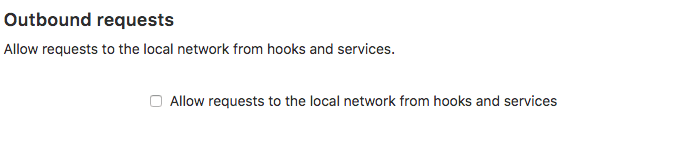
\includegraphics[width=13cm]{img/webhook_gitlab_setup.png}\\
			\caption[Webhook, GitLab]{Configurazione webhook con destinazione in rete locale}
		\end{figure}
		Ulteriori informazioni al riguardo possono essere trovate nella pagina\footnote{\url{https://docs.gitlab.com/ee/security/webhooks.html}} relativa a questo argomento sulla parte del sito relativa alla documentazione di GitLab.
		\subparagraph{Configurazione destinazione}
		Successivamente si può aggiungere indirizzo di destinazione un webhook al progetto andando sulle impostazioni:
		\begin{center}
			\texttt{Settings > Integrations}
		\end{center}
		Da qui si possono selezionare gli eventi di interessi per i quali i webhook verranno attivati (attenzione: \progetto~non supporta tutti gli eventi, solamente quelli richiesti da \II).
		Nel campo relativo all'URL di destinazione inserire l'indirizzo, con relativa porta (nel nostro caso quella specificata nella Tabella 2), su cui il Producer GitLab è in ascolto.
		\subparagraph{Eventi supportati}
		Per GitLab gli eventi supportati sono:
		\begin{itemize}
			\item Push events
			\item Comments
			\item Issues events
		\end{itemize}


---


	%TODO RIVEDERE
	La configurazione dei consumer e dei producer sono composte da file json contenti informazioni come ad esempio la mail di invio e la password relativa utilizzate per accedere al server mail.
	Queste possono essere modificate in modo tale da rispecchiare la configurazione che si vuole usare.
	
\subsection{Servizi aggiuntivi}
Aggiungere servizio necessario per il monitoraggio di kafka
Altri servizi per monitoraggio ?
    \section{Utilizzo di Butterfly}\label{utilizzo}

\subsection{Gestore Personale}

Il Gestore Personale è la componente principale di \progetto\ e si può suddividere in due sotto-componenti principali:

\begin{itemize}
    \item Interfaccia utente a sua volta divisa in
    \begin{itemize}
    	\item Interfaccia per amministratore
    	\item Interfaccia per utente normale
    \end{itemize}
    \item Message processor, che contiene la logica di business di \progetto
\end{itemize}

Il secondo punto non è di pertinenza di questo manuale (ma del \MSd), in quanto l'utente non lo usa direttamente, per cui verrà solamente discusso l'utilizzo del sistema tramite l'interfaccia utente. \par
L'inserimento della figura dell'amministratore, non presente nel \textit{Manuale Sviluppatore V1.0.0\ped{\tiny{D}}}, è giustificata in \textit{VE\_2019-04-26\ped{\tiny{D}}}.

\subsubsection{Interfaccia utente}
Le seguenti opzioni del Gestore Personale sono accessibili da ogni tipo utente, perciò anche da quelli coi privilegi di amministratore.

\paragraph{Accesso}
È possibile effettuare l'accesso all'interno del sistema tramite il link del container sul quale è in esecuzione, specificato nella configurazione effettuata precedentemente.
Per effettuare correttamente l'accesso è necessario l'inserimento del proprio ID Telegram o Email con il quale si è iscritti nel sistema.
\begin{figure}[H]
	\centering
	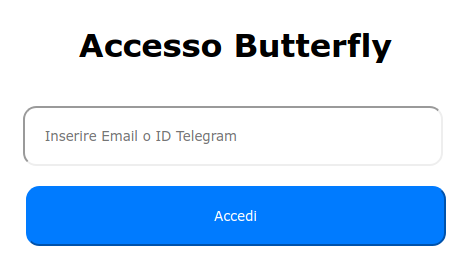
\includegraphics[width=9cm]{img/accesso_1.png}
	\caption{Form di accesso al sistema}
\end{figure}
In caso l'identificativo inserito non fosse valido, e non corrispondesse quindi a un match nel database, verrà mostrato all'utente un messaggio di errore.
\begin{figure}[H]
	\centering
	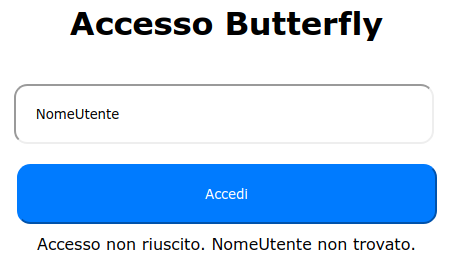
\includegraphics[width=9cm]{img/accesso_2.png}
	\caption{Messaggio di errore durante accesso al sistema}
\end{figure}

Nel caso in cui un utente cerchi di accedere ad una sezione, ma senza aver effettuato l'accesso, questo verrà rimandato alla pagina di accesso.\par
Se un utente iscritto correttamente nel sistema ha registrato precedentemente sia indirizzo Email che ID Telegram, allora può accedere utilizzando indipendentemente il primo o il secondo.
In cima alla pagina, per identificare l'utente che ha acceduto, viene mostrato l'ID Telegram o la mail con cui si ha acceduto.

\paragraph{Pannello di controllo}
Dopo aver effettuato l'accesso al sistema, si viene rimandati alla pagina relativa al pannello di controllo che contiene i comandi principali per la navigazione del sito e le operazioni che un utente può eseguire.
Le sezioni a cui si può navigare dal pannello di controllo sono:
\begin{itemize}
	\item Modifica dei propri dati
	\item Modifica delle proprie preferenze
	\item Uscita dal sistema (logout)
\end{itemize}
\begin{figure}[H]
	\centering
	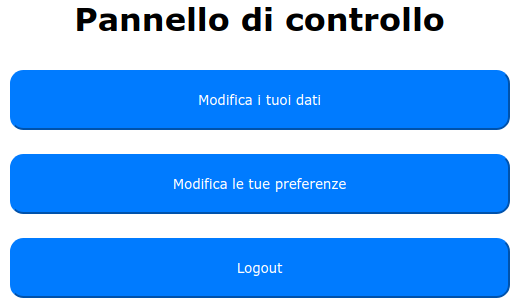
\includegraphics[width=10cm]{img/user_panel_1.png}
	\caption{Pannello di controllo per utente generico}
\end{figure}

\paragraph{Modifica preferenze}\label{preferenze}
La modifica delle preferenze è possibile solamente per utenti già iscritti ed autenticati nel sistema.
È raggiungibile tramite il pannello di controllo sotto la voce ``Modifica le tue preferenze''.
In questa sezione si possono trovare le principali impostazioni del sistema dal punto di vista dell'utente finale:
\begin{itemize}
	\item Lista dei progetti a cui si è iscritti
	\item Modifica della priorità assegnata ad un progetto che può essere:
	\begin{itemize}
        \item \textbf{Alta}: 1
        \item \textbf{Media}: 2
        \item \textbf{Bassa}: 3
    \end{itemize}
	\item Lista dei Topic (formati dall'insieme di label e keyword) disponibili e iscrizione o disiscrizione da questi, che vengono mostrati dinamicamente in base ai progetti a cui si è iscritti. L'inserimento per keyword d'interesse deve essere fatta in modo testuale e la loro divisione viene riconosciuta attraverso una ``,'' 
	\item Modifica dei progetti d'interesse (aggiunta o rimozione dei progetti dalle proprie preferenze)
	\item Inserimento dei giorni di indisponibilità da calendario
	\item Impostazione delle due piattaforme di messaggistica (Email o Telegram) su cui ricevere le notifiche. \'E possibile scegliere solo una delle due piattaforme di messaggistica
\end{itemize}
Le ``label'' non sono modificabili in quanto vengono aggiornate solamente da una componente del Gestore Personale che le memorizza quando avvengono \gloss{update} alle issue relative ai progetti.
Le ``keyword'' invece, sono formate da una lista di parole che possono essere contenute nei messaggi di push di GitLab e di cui si è interessati a ricevere notifiche.
\begin{figure}[H]
	\centering
	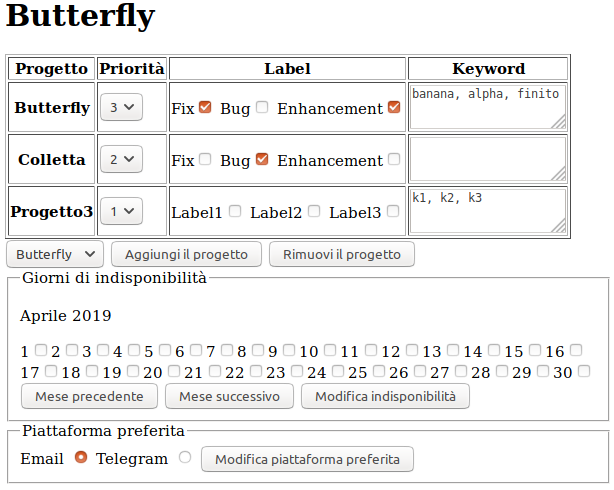
\includegraphics[width=\textwidth]{img/preferenze_1.png}
	\caption{Interfaccia modifica preferenze}
\end{figure}

\paragraph{Modifica dei propri dati}
La modifica dei propri dati è possibile attraverso la sezione ``Modifica i tuoi dati'' accessibile dal pannello di controllo.
Qui un utente può modificare i dati inseriti dall'amministratore in fase di registrazione.
\begin{figure}[H]
	\centering
	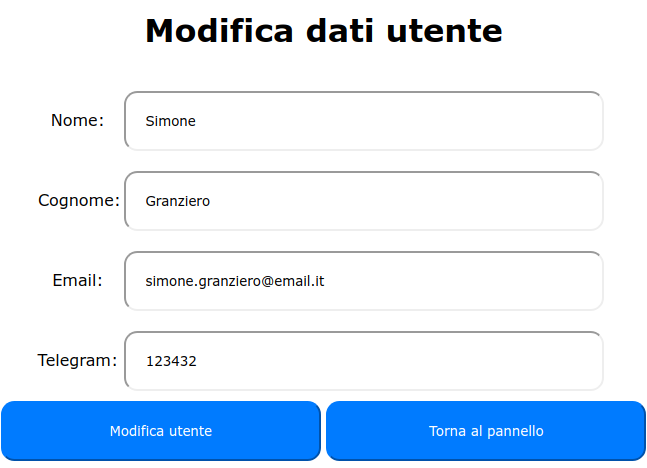
\includegraphics[width=10cm]{img/modifica_1.png}
	\caption{Modifica dei dati di un utente}
\end{figure}
Nel caso questi fossero già associati ad una persona iscritta a \progetto, verrà visualizzato un messaggio di errore. \par
Per quanto riguarda l'inserimento dell'ID Telegram, questo non deve essere nella forma \texttt{@nome\_utente}, ma bensì numerico. Per poterlo ottenere consigliamo l'utilizzo del bot Telegram ``MyIDBot\footnote{\url{https://telegram.me/storebot?start=myidbot}}'' dandogli il comando \texttt{/getid}.

\paragraph{Uscita dal sistema}
Per effettuare il logout dal sistema, cliccare sul bottone ``Logout'' presente nel pannello di controllo.

\subsubsection{Interfaccia amministratore}
All'interno dell'applicazione \progetto, gli utenti con i permessi di amministratore potranno eseguire le stesse azioni di un utente normale e in più gestire l'insieme degli utenti iscritti al sistema. Il sistema di accesso per l'utente amministratore non differisce da quello per gli altri utenti.

\paragraph{Pannello di controllo}
Dopo aver effettuato l'accesso al sistema, si viene rimandati alla pagina relativa al pannello di controllo che contiene i comandi principali per la navigazione del sito e le operazioni che un utente può eseguire.
Le sezioni a cui si può navigare dal pannello di controllo sono:
\begin{itemize}
    \item Inserimento di un nuovo utente
    \item Rimozione di un utente
    \item Visualizzazione degli utenti iscritti
    \item Rimozione di un progetto
    \item Visualizzazione dei progetti
    \item Modifica dei propri dati
    \item Modifica delle proprie preferenze
	\item Uscita dal sistema (logout)
\end{itemize}
\begin{figure}[H]
    \centering
    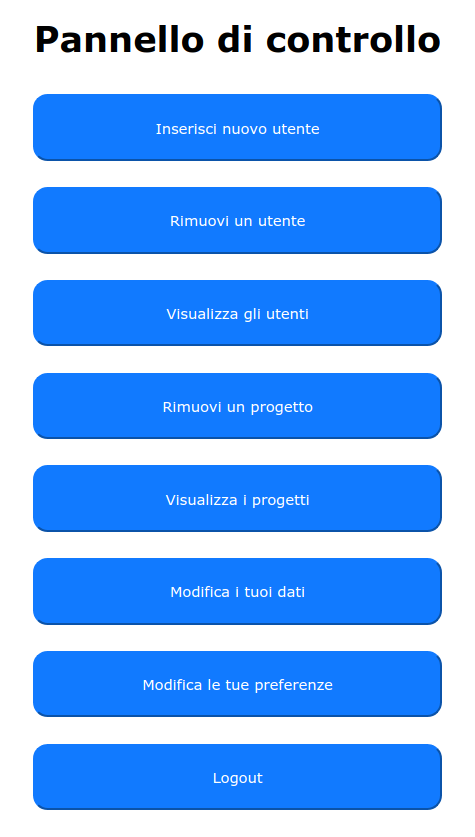
\includegraphics[width=10cm]{img/admin_panel_1.png}
    \caption{Pannello di controllo per utente con privilegi di amministratore}
\end{figure}

\paragraph{Iscrizione a Butterfly}\label{Iscrizione}
L'iscrizione di un nuovo utente al sistema \progetto\ è permessa solamente all'utente amministratore.
La sezione di inserimento di un nuovo utente è raggiungibile dal pannello di controllo e prevede l'inserimento dei seguenti dati:
\begin{itemize}
	\item Nome
	\item Cognome
	\item Email
	\item Telegram
\end{itemize}
\begin{figure}[H]
	\centering
	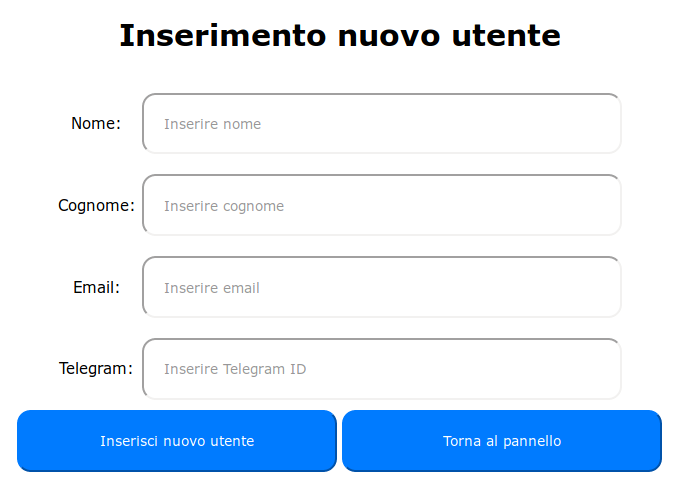
\includegraphics[width=13cm]{img/inserimento_1.png}
	\caption{Interfaccia inserimento nuovo utente}
\end{figure}

È necessario inserire almeno un campo a scelta tra Email e Telegram.
Nel caso questi fossero già associati ad un utente iscritto a \progetto\ verrà visualizzato un messaggio di errore.

\paragraph{Rimozione di un utente}\label{Rimozione}
Viene data la possibilità di rimuovere un utente dal sistema solamente all'amministratore.
La rimozione è possibile attraverso la sezione ``Rimuovi un utente'' accessibile dal pannello di controllo.
\begin{figure}[H]
	\centering
	
\includegraphics[width=12cm]{img/rimozione_1.png}
	\caption{Interfaccia rimozione di un utente}
\end{figure}

\paragraph{Visualizzazione utenti} \label{VisUtenti}
Un utente amministratore ha la possibilità di vedere la lista di tutti gli utenti iscritti al sistema e i relativi progetti a cui sono interessati.
Per ogni progetto viene inoltre riportata la priorità che ha per l'utente, le labels e la keywords d'interesse.
La visualizzazione avviene attraverso la sezione ``Visualizza gli utenti'' accessibile dal pannello di controllo.
\begin{figure}[H]
	\centering
	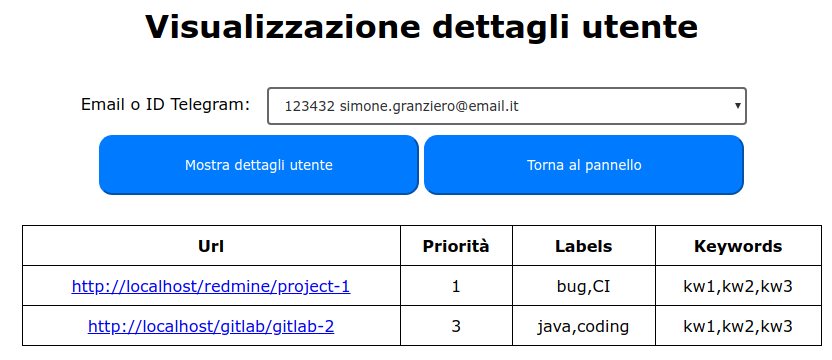
\includegraphics[width=12cm]{img/user_details.png}
	\caption{Interfaccia visualizzazione degli utenti}
\end{figure}

\paragraph{Rimozione di un progetto}
I progetti provenienti da GitLab o Redmine vengono aggiunti in automatico al sistema e la loro gestione (intesa come creazione e modifica) non è competenza degli utenti. Perciò i progetti possono solo essere aggiunti o rimossi dalle preferenze di un utente, oppure rimossi completamente dal sistema nel momento in cui questi, ad esempio, vengono chiusi nelle relative applicazioni di provenienza. \par
Per rimuovere un progetto dal sistema, l'interfaccia dell'amministratore possiede un'apposita pagina chiamata ``Rimuovi un  progetto'' dove è possibile selezionare i progetti da rimuovere.
\begin{figure}[H]
    \centering
	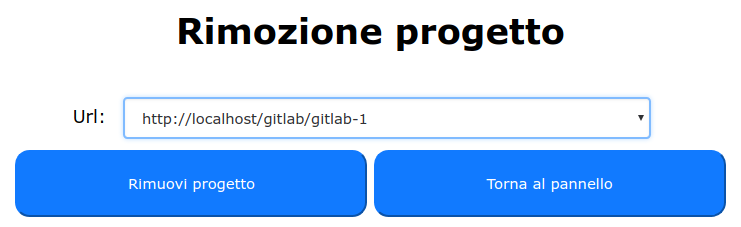
\includegraphics[width=12cm]{img/rimozioneprog.png}
	\caption{Interfaccia rimozione di un progetto }
\end{figure}

\paragraph{Visualizzazione dei progetti}
Un utente amministratore ha la possibilità di vedere la lista di tutti i progetti presenti nel sistema. Di ognuno viene mostrata la url identificativa, il nome, l'applicazione di provenienza e i topics rilevati relativi al progetto.
La visualizzazione avviene attraverso la sezione ``Visualizza i progetti'' accessibile dal pannello di controllo.
\begin{figure}[H]
	\centering
	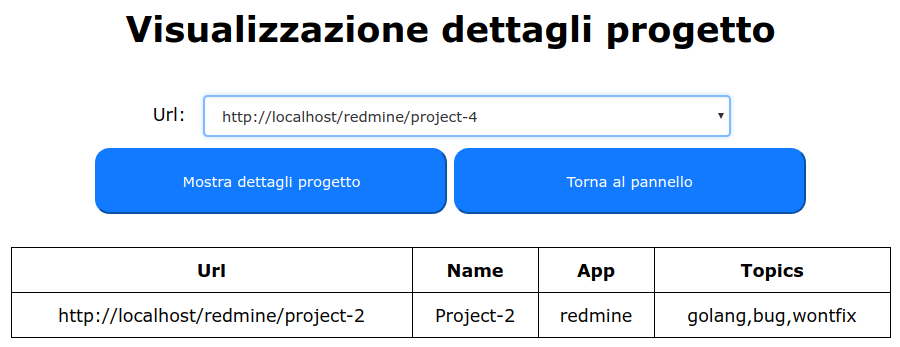
\includegraphics[width=12cm]{img/visualizzaprog.png}
	\caption{Interfaccia visualiazzione dei progetti}
\end{figure}


\subsection{API Rest}\label{APIRest}
\newcommand{\homeUrl}{home\_url}

Per la gestione delle risorse di \progetto\ abbiamo utilizzato lo standard architetturale delle API Rest.
Nelle sezioni successive viene descritto come interagire con le API fornite dal sistema.
Il \gloss{root path} sottinteso sarà sempre \texttt{\homeUrl/api/v1/}.
Ad esempio, per effettuare la GET dell'user \texttt{@user1}, l'indirizzo sarà:
\begin{center}
    \texttt{GET \homeUrl/api/v1/user/@user1}
\end{center}

\subsubsection{User}

\texttt{User} è la risorsa utente.
È possibile visualizzare, aggiungere, modificare o rimuovere gli utenti tramite una semplice
richiesta HTTP.

\paragraph{Visualizzazione}
È possibile visualizzare i dati di un utente tramite la richiesta
    \begin{center}
        \texttt{GET  /user/<id>}
    \end{center}

    \subparagraph{Esempio di input}
    Un esempio di richiesta è
        \begin{center}
            \texttt{GET  /user/abcd@bc.it}
        \end{center}
    senza alcun dato nel \gloss{payload} della richiesta.

    \subparagraph{Esempio di output}
    In caso la richiesta vada a buon fine, un esempio di output è
    \begin{lstlisting}[language = json]
{
    "_id": {
        "$oid": "5cd07bb9c331755af7f5ea00"
    },
    "name": "Mattia",
    "surname": "Cruciani",
    "email": "abcd@bc.it",
    "telegram": "1234",
    "admin": false,
    "preference": "email",
    "irreperibilita": [
        {
            "$date": "2018-12-05"
        },
        {
            "$date": "2019-04-08"
        },
        {
            "$date": "2019-04-15"
        },
        {
            "$date": "2019-04-07"
        },
        {
            "$date": "2019-06-07"
        },
        {
            "$date": "2019-06-08"
        },
        {
            "$date": "2019-06-09"
        }
    ],
    "projects": [
        {
            "url": "http://localhost/gitlab/gitlab-2",
            "priority": 2,
            "topics": [
                "java",
                "coding",
                "criptovaluta"
            ],
            "keywords": [
                "kw1",
                "kw2",
                "kw3"
            ]
        }
    ]
}
    \end{lstlisting}

    Nel caso l'utente richiesto non venga trovato, verrà restituito il seguente messaggio
    \begin{lstlisting}[language = json]
{
    "error": "Utente inesistente."
}
    \end{lstlisting}

\paragraph{Inserimento}
È possibile inserire un nuovo utente tramite la richiesta:
    \begin{center}
        \texttt{POST /user}
    \end{center}

È inoltre possibile dare i seguenti campi di tipo stringa alla richiesta, per aggiungere in fase di creazione i dati:
\begin{itemize}[noitemsep]
    \item \texttt{name}
    \item \texttt{surname}
    \item \texttt{telegram}
    \item \texttt{email}
\end{itemize}
Almeno uno tra i campi \texttt{Email} e \texttt{ID Telegram} vanno fornite insieme al payload.

    \subparagraph{Esempio di input}
    Un esempio di richiesta è
        \begin{center}
            \texttt{POST  /user}
        \end{center}
    con i seguenti dati nel corpo della richiesta
    \begin{lstlisting}[language = json]
{
    "name": "Matteo",
    "surname": "Marchiori",
    "email": "matteo.marchiori97@gmail.com",
    "telegram": "123456"
}
    \end{lstlisting}


    \subparagraph{Esempio di output}
    In caso la richiesta vada a buon fine, verrà restituito il seguente messaggio
    \begin{lstlisting}[language = json]
{
    "ok": "Utente inserito correttamente"
}
    \end{lstlisting}

    Nel caso l'utente da inserire esista già, verrà restituito il seguente messaggio
    \begin{lstlisting}[language = json]
{
    "error": "L'utente inserito esiste già."
}
    \end{lstlisting}

    Nel caso non vengano inseriti almeno email o telegram, verrà restituito il seguente messaggio
    \begin{lstlisting}[language = json]
{
    "error": "Si prega di inserire almeno email o telegram per inserire l'utente."
}
    \end{lstlisting}

\paragraph{Modifica}

È possibile modificare un utente tramite la richiesta
\begin{center}
    \texttt{PUT /user/<id>}
\end{center}

È possibile dare i seguenti campi di tipo stringa alla richiesta, per aggiungere in fase di modifica i dati:
\begin{itemize}[noitemsep]
    \item \texttt{name}
    \item \texttt{surname}
    \item \texttt{telegram}
    \item \texttt{email}
\end{itemize}

    \subparagraph{Esempio di input}
    Un esempio di richiesta è
    \begin{center}
	    \texttt{PUT /user/1234}
    \end{center}
    con i seguenti dati nel corpo della richiesta
	\begin{lstlisting}[language = json]
{
    "name": "Marco",
    "surname": "Rossi",
    "telegram": "1235"
}
    \end{lstlisting}

    \subparagraph{Esempio di output}
    In caso la richiesta vada a buon fine, verrà restituito il seguente messaggio
	\begin{lstlisting}[language = json]
{
    "ok": "Utente modificato correttamente"
}
	\end{lstlisting}

	In caso non vengano forniti almeno Email o ID Telegram, verrà restituito il seguente messaggio
	\begin{lstlisting}[language = json]
{
    "error": "Si prega di inserire almeno email o telegram per modificare l'utente."
}
	\end{lstlisting}

	In caso almeno uno degli identificativi forniti coincida con quello di un altro utente, verrà restituito il seguente messaggio
	\begin{lstlisting}[language = json]
{
    "error": "I dati inseriti confliggono con altri già esistenti."
}
	\end{lstlisting}

\paragraph{Rimozione}

È possibile rimuovere un utente dal sistema \progetto\ con la richiesta
\begin{center}
    \texttt{DELETE /user/<id>}
\end{center}

Se il campo \texttt{<id>} corrisponde a un ID presente nel sistema, esso verrà rimosso.

    \subparagraph{Esempio di input}
    Un esempio di richiesta è
    \begin{center}
        \texttt{DELETE  /user/abcd@bc.it}
    \end{center}
    senza alcun dato nel \gloss{payload} della richiesta.

    \subparagraph{Esempio di output}
    In caso la richiesta vada a buon fine, verrà restituito il seguente messaggio
	\begin{lstlisting}[language = json]
{
    "ok": "Utente rimosso correttamente"
}
	\end{lstlisting}


\paragraph{Riepilogo}

\begin{table}[H]
    \begin{paddedtablex}[1.3]{\textwidth}{cYY}
        \thead{Metodo HTTP} & \thead{URI} & \thead{Action}\\\toprule
        \texttt{GET} & \texttt{/user/<id>} & Restituisce un payload in JSON dell'utente che corrisponde a \texttt{<id>}\\
        \texttt{POST} & \texttt{/user} & Inserisce un nuovo utente. È necessario fornire uno tra i campi telegram o email\\
        \texttt{PUT} & \texttt{/user/<id>} & Modifica l'utente corrispondente a \texttt{<id>} con i campi passati nella richiesta\\
        \texttt{DELETE} & \texttt{/user/<id>} & Elimina l'utente corrispondente a \texttt{<id>} dal sistema\\
        \bottomrule
    \end{paddedtablex}
    \caption{Riepilogo delle Rest API per la risorsa User}
\end{table}


\subsubsection{Project}
Project è la risorsa relativa ai progetti. È possibile visualizzare o rimuovere i progetti tramite una semplice richiesta HTTP.

\paragraph{Visualizzazione}
È possibile visualizzare i progetti tramite la richiesta
    \begin{center}
        \texttt{GET /project/<id>}
    \end{center}
Se il campo \texttt{<id>} corrisponde a un progetto, verranno mostrati i dati relativi a tale progetto.

    \subparagraph{Esempio di input}
    Un esempio di richiesta è
        \begin{center}
            \texttt{GET /project/http://localhost/gitlab/gitlab-2}
        \end{center}
    senza alcun dato nel \gloss{payload} della richiesta.

    \subparagraph{Esempio di output}
    In caso la richiesta vada a buon fine, un esempio di output è
    \begin{lstlisting}[language = json]
{
    "_id": {
        "$oid": "5cd1b509c331756598e9c00b"
    },
    "url": "http://localhost/gitlab/gitlab-2",
    "name": "Gitlab-2",
    "app": "gitlab",
    "topics": [
        "java",
        "coding",
        "enhancement",
        "bug"
    ]
}
	\end{lstlisting}

	In caso il progetto richiesto non esista, verrà restituito il seguente messaggio
    \begin{lstlisting}[language = json]
{
    "error": "Progetto inesistente."
}
	\end{lstlisting}


\paragraph{Rimozione}

È possibile rimuovere un progetto dal sistema Butterfly con la richiesta
\begin{center}
    \texttt{DELETE /project/<id>}
\end{center}

Se il campo \texttt{<id>} corrisponde a un progetto, esso verrà rimossa dal sistema.

    \subparagraph{Esempio di input}
    Un esempio di richiesta è
    \begin{center}
	    \texttt{DELETE /project/http://localhost/gitlab/gitlab-2}
    \end{center}
    senza alcun dato nel \gloss{payload} della richiesta.

    \subparagraph{Esempio output}
    In caso la richiesta vada a buon fine, verrà restituito il seguente messaggio
    \begin{lstlisting}[language = json]
{
    "ok": "Progetto rimosso correttamente"
}
    \end{lstlisting}

\paragraph{Riepilogo}

\begin{table}[H]
    \begin{paddedtablex}[1.3]{\textwidth}{cYY}
        \thead{Metodo HTTP} & \thead{URI} & \thead{Action}\\\toprule
        \texttt{GET} & \texttt{/project/<id>} & Restituisce un payload in JSON del progetto corrispondente a \texttt{<id>}\\
        \texttt{DELETE} & \texttt{/project/<id>} & Elimina il progetto corrispondente a \texttt{<id>} dal sistema \\
        \bottomrule
    \end{paddedtablex}
    \caption{Riepilogo delle Rest API per la risorsa Project}
\end{table}


\subsubsection{Preference}

\texttt{Preference} è la risorsa preferenza.
È possibile modificare le preferenze degli utenti tramite questa risorsa.

\paragraph{Inserimento}
È possibile inserire un nuovo progetto tra le preferenze tramite la richiesta:
    \begin{center}
        \texttt{POST /preference}
    \end{center}

È inoltre richiesto dare i seguenti campi di tipo stringa alla richiesta, per aggiungere in fase di creazione i dati:
\begin{itemize}[noitemsep]
    \item \texttt{user}
    \item \texttt{project}
\end{itemize}

    \subparagraph{Esempio di input}
    Un esempio di richiesta è
        \begin{center}
            \texttt{POST  /preference}
        \end{center}
    con i seguenti dati nel corpo della richiesta
    \begin{lstlisting}[language = json]
{
    "user": "1234",
    "project": "http://localhost/redmine/project-2"
}
    \end{lstlisting}


    \subparagraph{Esempio di output}
    In caso la richiesta vada a buon fine, verrà restituito il seguente messaggio
    \begin{lstlisting}[language = json]
{
    "ok": "Preferenza aggiunta correttamente"
}
    \end{lstlisting}

    Nel caso il progetto esista già tra le preferenze, o non esista l'utente specificato, verrà restituito il seguente messaggio
    \begin{lstlisting}[language = json]
{
    "error": "Progetto già presente o utente inesistente."
}
    \end{lstlisting}

    Nel caso non venga specificato il progetto, verrà restituito il seguente messaggio
    \begin{lstlisting}[language = json]
{
    "error": "Nessun progetto selezionato o progetto inesistente."
}
    \end{lstlisting}


\paragraph{Modifica}

È possibile modificare le preferenze di un utente tramite la richiesta
\begin{center}
    \texttt{PUT /preference/<id>}
\end{center}

Le preferenze hanno i seguenti tipi:
\begin{itemize}[noitemsep]
    \item \texttt{topics}
    \item \texttt{irreperibilita}
    \item \texttt{piattaforma}
\end{itemize}

Il tipo di preferenza va indicato nel payload usando il campo ``tipo''.

In base al tipo di preferenza è possibile dare i seguenti campi di tipo stringa alla richiesta, per aggiungere in fase di modifica i dati:

\begin{itemize}[noitemsep]
    \item \texttt{topics}
    \begin{itemize}
        \item \texttt{project}
        \item \texttt{priority}
        \item \texttt{topics}
        \item \texttt{keywords}
    \end{itemize}
    \item \texttt{irreperibilita}
    \begin{itemize}
        \item \texttt{giorni}
    \end{itemize}
    \item \texttt{piattaforma}
    \begin{itemize}
        \item \texttt{platform}
    \end{itemize}
\end{itemize}

    \subparagraph{Esempio di input}
    Un esempio di richiesta è
    \begin{center}
	    \texttt{PUT /preference/1234}
    \end{center}
    con i seguenti dati nel corpo della richiesta
	\begin{lstlisting}[language = json]
{
    "tipo": "topics",
    "project": "http://localhost/redmine/project-2",
    "priority": "2",
    "topics": "['bug','feature','banana']",
    "keywords": "['keyword','42']"
}
    \end{lstlisting}

    Un esempio per l'irreperibilità è
    \begin{center}
	    \texttt{PUT /preference/1234}
    \end{center}
    con i seguenti dati nel corpo della richiesta
	\begin{lstlisting}[language = json]
{
    "tipo": "irreperibilita",
    "giorni": "['2019-05-25','2019-05-26','2019-06-01']"
}
    \end{lstlisting}

    Invece un esempio per modificare la piattaforma preferita di ricezione dei messaggi è
    \begin{center}
	    \texttt{PUT /preference/1234}
    \end{center}
    con i seguenti dati nel corpo della richiesta
	\begin{lstlisting}[language = json]
{
    "tipo": "piattaforma",
    "platform": "email"
}
    \end{lstlisting}

    \subparagraph{Esempio di output}
    In caso la richiesta vada a buon fine, verrà restituito il seguente messaggio
	\begin{lstlisting}[language = json]
{
    "ok": "Preferenza modificata correttamente"
}
	\end{lstlisting}

	Nel caso si stia cercando di impostare la piattaforma preferita non avendo registrato l'account verrà restituito uno dei seguenti messaggi
	\begin{lstlisting}[language = json]
{
    "error": "Telegram non presente nel sistema."
}
	\end{lstlisting}

	oppure

	\begin{lstlisting}[language = json]
{
    "error": "Email non presente nel sistema."
}
	\end{lstlisting}

\paragraph{Rimozione}

È possibile rimuovere un progetto dalle preferenze di un utente con la richiesta
\begin{center}
    \texttt{DELETE /preference/<id>}
\end{center}

Se il campo \texttt{<id>} corrisponde a un utente, il progetto verrà rimosso dalle sue preferenze.

    \subparagraph{Esempio di input}
    Un esempio di richiesta è
    \begin{center}
	    \texttt{DELETE /preference/1234}
    \end{center}
    con i seguenti dati nel corpo della richiesta
	\begin{lstlisting}[language = json]
{
    "project": "http://localhost/redmine/project-2"
}
    \end{lstlisting}

    \subparagraph{Esempio output}
    In caso la richiesta vada a buon fine, verrà restituito il seguente messaggio
    \begin{lstlisting}[language = json]
{
    "ok": "Preferenza rimossa correttamente."
}
    \end{lstlisting}

    In caso non venga fornito un progetto nella richiesta, verrà restituito il messaggio
    \begin{lstlisting}[language = json]
{
    "error": "Nessun progetto selezionato o progetto inesistente."
}
    \end{lstlisting}

    In caso l'utente non abbia il progetto specificato tra le preferenze o non esista l'utente specificato verrà restituito il messaggio
    \begin{lstlisting}[language = json]
{
    "error": "Progetto non presente nelle preferenze o utente inesistente."
}
    \end{lstlisting}

\paragraph{Riepilogo}

\begin{table}[H]
    \begin{paddedtablex}[1.3]{\textwidth}{cYY}
        \thead{Metodo HTTP} & \thead{URI} & \thead{Action}\\\toprule
        \texttt{POST} & \texttt{/preference} & Aggiunge la preferenza all'utente specificato nella richiesta con i campi passati nella richiesta\\
        \texttt{PUT} & \texttt{/preference/<id>} & Modifica la preferenza dell'utente corrispondente a \texttt{<id>} con i campi passati nella richiesta\\
        \texttt{DELETE} & \texttt{/preference/<id>} & Rimuove la preferenza dell'utente corrispondente a \texttt{<id>}\\
        \bottomrule
    \end{paddedtablex}
    \caption{Riepilogo delle Rest API per la risorsa Preference}
\end{table}


\newpage

\subsection{Piattaforma di messaggistica}

\subsubsection{Email}

Per ricevere i messaggi di Butterfly tramite Email, è sufficiente fornire tramite l'interfaccia del Gestore Personale l'Email sulla quale si vuole ricevere la notifica.

\begin{figure}[H]
	\centering
	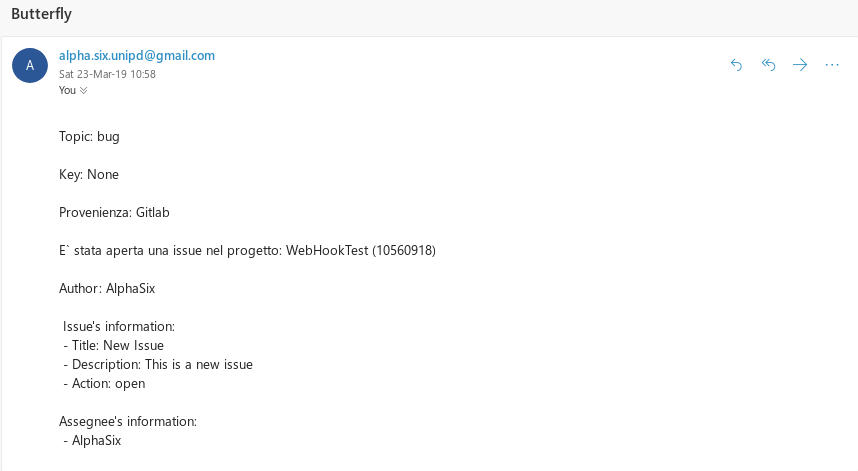
\includegraphics[width=\textwidth]{img/notifica_email_1.png}
	\caption{Formato dell' Email ricevuta da un utente finale}
\end{figure}

\subsubsection{Telegram}

Per ricevere le notifiche via Telegram, è necessario fare un passaggio addizionale: va fornita l'autorizzazione al bot per poter inviare messaggi agli utenti.
Il bot è raggiungibile al seguente link:
\begin{center}
    \url{http://t.me/ButterflyBot}
\end{center}

Dare il comando \texttt{/start} per dare l'autorizzazione di inoltro dei messaggi al bot.
È necessario inoltre aggiungere tramite l'interfaccia del Gestore Personale il proprio account Telegram.
In qualsiasi momento sarà possibile bloccare il bot in caso non si vogliano più ricevere messaggi relativi a Butterfly su Telegram, tramite le funzionalità dell'applicazione.
\begin{figure}[H]
	\centering
	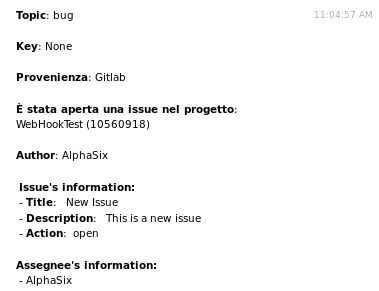
\includegraphics[width=9cm]{img/notifica_telegram_1.png}
	\caption{Formato del messaggio Telegram ricevuto da un utente finale}
\end{figure}
Nel caso in cui si volesse utilizzare un altro bot, i passaggi da seguire possono essere trovati sulla pagina apposita della documentazione di Telegram\footnote{\url{https://core.telegram.org/bots}}.
Per comunicare con questo bisogna modificare la variabile di ambiente \texttt{BUTTERFLY\_CONSUMER\_TELEGRAM\_BOT} che rappresenta il \texttt{token} univoco del nuovo bot, come descritto in \S\ref{var_consumer}.

    \section{Segnalazione problematiche}

Nel caso dovessero venire riscontrati bug o problematiche relative a \progetto, si prega di segnalarlo tramite una delle seguenti procedure:
\begin{itemize}
    \item Inviare una mail all'indirizzo \href{mailto:alpha.six.unipd@gmail.com}{alpha.six.unipd@gmail.com}
    \item Aprire una issue nel progetto \progetto\ su GitHub, descrivendo nel modo più accurato possibile il problema e come riprodurlo.
    % TODO nella seconda versione da rilasciare mettere un footnote con il link al progetto in github
\end{itemize}


    \appendix
    \section{Glossario}\label{glossario}

% \lettera{A} % Da mettere le lettere?

\parola{Rancher}{text}

\parola{Webhook}{text text text text text text}


\end{document}
